\begin{figure}[!]
    \centering
    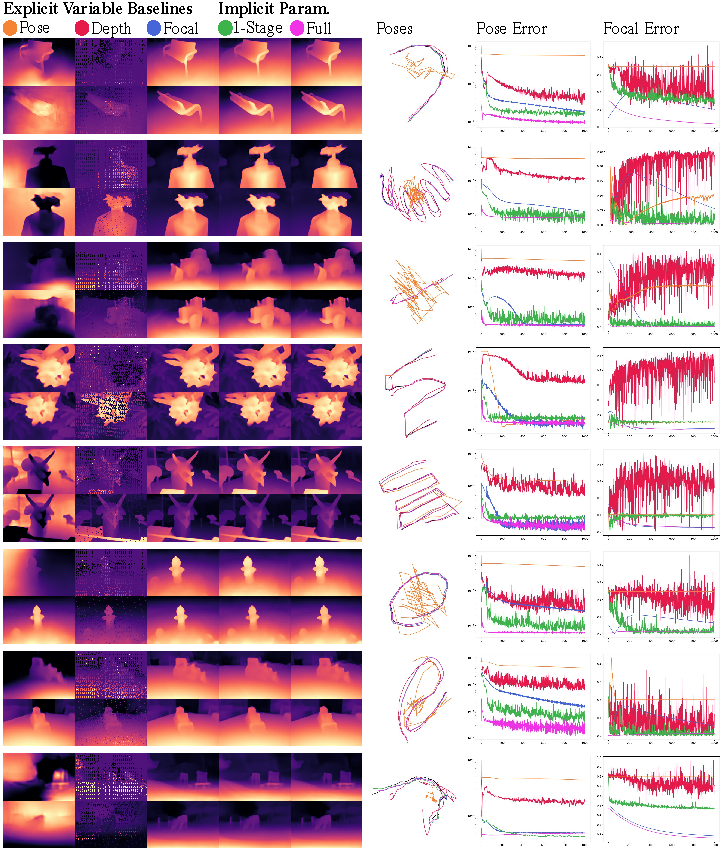
\includegraphics[width=\linewidth,]{figures/pdfs/source_matrix_large_compressed.pdf}
    \caption{\textbf{Pose and Geometry Convergence for Free-Variable vs. Proposed Parameterizations.}
    We plot poses, depths, focal lengths, and pose error (ATE) obtained with our proposed parameterizations (``Full'') vs. those obtained with free-variable parameterizations at various optimization steps. With our proposed reparameterizations (``Full'') as a baseline, we ablate either depth, focal length, or poses as free-variable optimizations and plot the resulting optimizations' pose and depth estimates. For instance, ``Depth'' corresponds to making the depth an explicit free-variable in the optimization. Using pose-as-variable and depth-as-variable often lead to ``hollow-face'' geometry, where the geometry is effectively inverted but still mostly satisfies the optical flow constraints. We also show results from a single-stage FlowMap pipeline, which only uses the implicit parameterization of intrinsics rather than switching to regressed intrinsics halfway through optimization. Note that the plotted lines for ``Full'' are initialized with the results of ``1-Stage'' and represent the second stage (explicit focal length) of FlowMap optimization.}
    \label{fig:convergence}
\end{figure}
